\documentclass[a4paper]{article}
\usepackage{hyperref}
\hypersetup{
  pdftitle={HW03},
  pdfauthor={Yin Yu},
  colorlinks=true,
  linkcolor=blue,
  citecolor=cyan
}
\usepackage{amsmath}
\usepackage{listings}
\usepackage{color}
\usepackage{xcolor}
\usepackage{fullpage}
\usepackage{graphicx}
\usepackage[all,pdf]{xy}

\definecolor{mygreen}{rgb}{0,0.6,0}
\definecolor{mygray}{rgb}{0.5,0.5,0.5}
\definecolor{mymauve}{rgb}{0.58,0,0.82}

\lstset{
  backgroundcolor=\color{white},
  basicstyle=\footnotesize\ttfamily,     
  breakatwhitespace=false,      
  breaklines=true,              
  captionpos=t,   
  commentstyle=\color{mygreen}, 
  escapeinside={\%*}{*)},
  frame=t,
  keepspaces=true,
  language=Bash,
  numbers=left,                   
  numbersep=5pt,                  
  numberstyle=\tiny\color{mygray},
  rulecolor=\color{black},        
  showspaces=false,               
  showstringspaces=false,         
  showtabs=false,                 
  stringstyle=\color{mymauve},
  tabsize=4,                  
  title=\lstname,
  xleftmargin=3em,
  xrightmargin=3em
}
\usepackage{caption}
\captionsetup[lstlisting]{
  font={tt,footnotesize}
}

\title{\textbf{HW03}}
\author{\texttt{PB13011038}\quad\textbf{Yin Yu}}
\date{\today}

\begin{document}

\maketitle

\begin{enumerate}

\item[3.3] Altogether $2^4=16$ two-input logic functions.

\item[3.6] See the table below. Z\,=\,A \verb+AND+ B.
\begin{center}
\begin{tabular}{cc|ccc}
\hline
A & B & C & D & Z \\
\hline
0 & 0 & 1 & 1 & 0 \\
0 & 1 & 1 & 0 & 0 \\
1 & 0 & 0 & 1 & 0 \\
1 & 1 & 0 & 0 & 1 \\
\hline
\end{tabular}
\end{center}

\item[3.7] There is short circuit when either A or B is 1 and the
  other is 0.

\item[3.14] It will have 1 output line and $\log_2{16}=4$ select
  lines.

\item[3.19] Figure 3.36 is a circuit that perform operations and
  figure 3.37 is has the storing functionality. That is, when A and B
  are both 1, in fig 3.36, D's value depends on what state A, B, C is
  in at present, but in fig 3.37, D's value depends on which of the
  input was 0 previously.

\item[3.24]
\begin{enumerate}
\item X controls which of B and C will be added to A. When X\,=\,0,
  $S=A+B$, otherwise $S=A+C$.
\item I constructed a four-bit adder/substractor as an
  example. Numbers are reprensented in 2's complement form. See the
  figure below.
  \begin{center}
  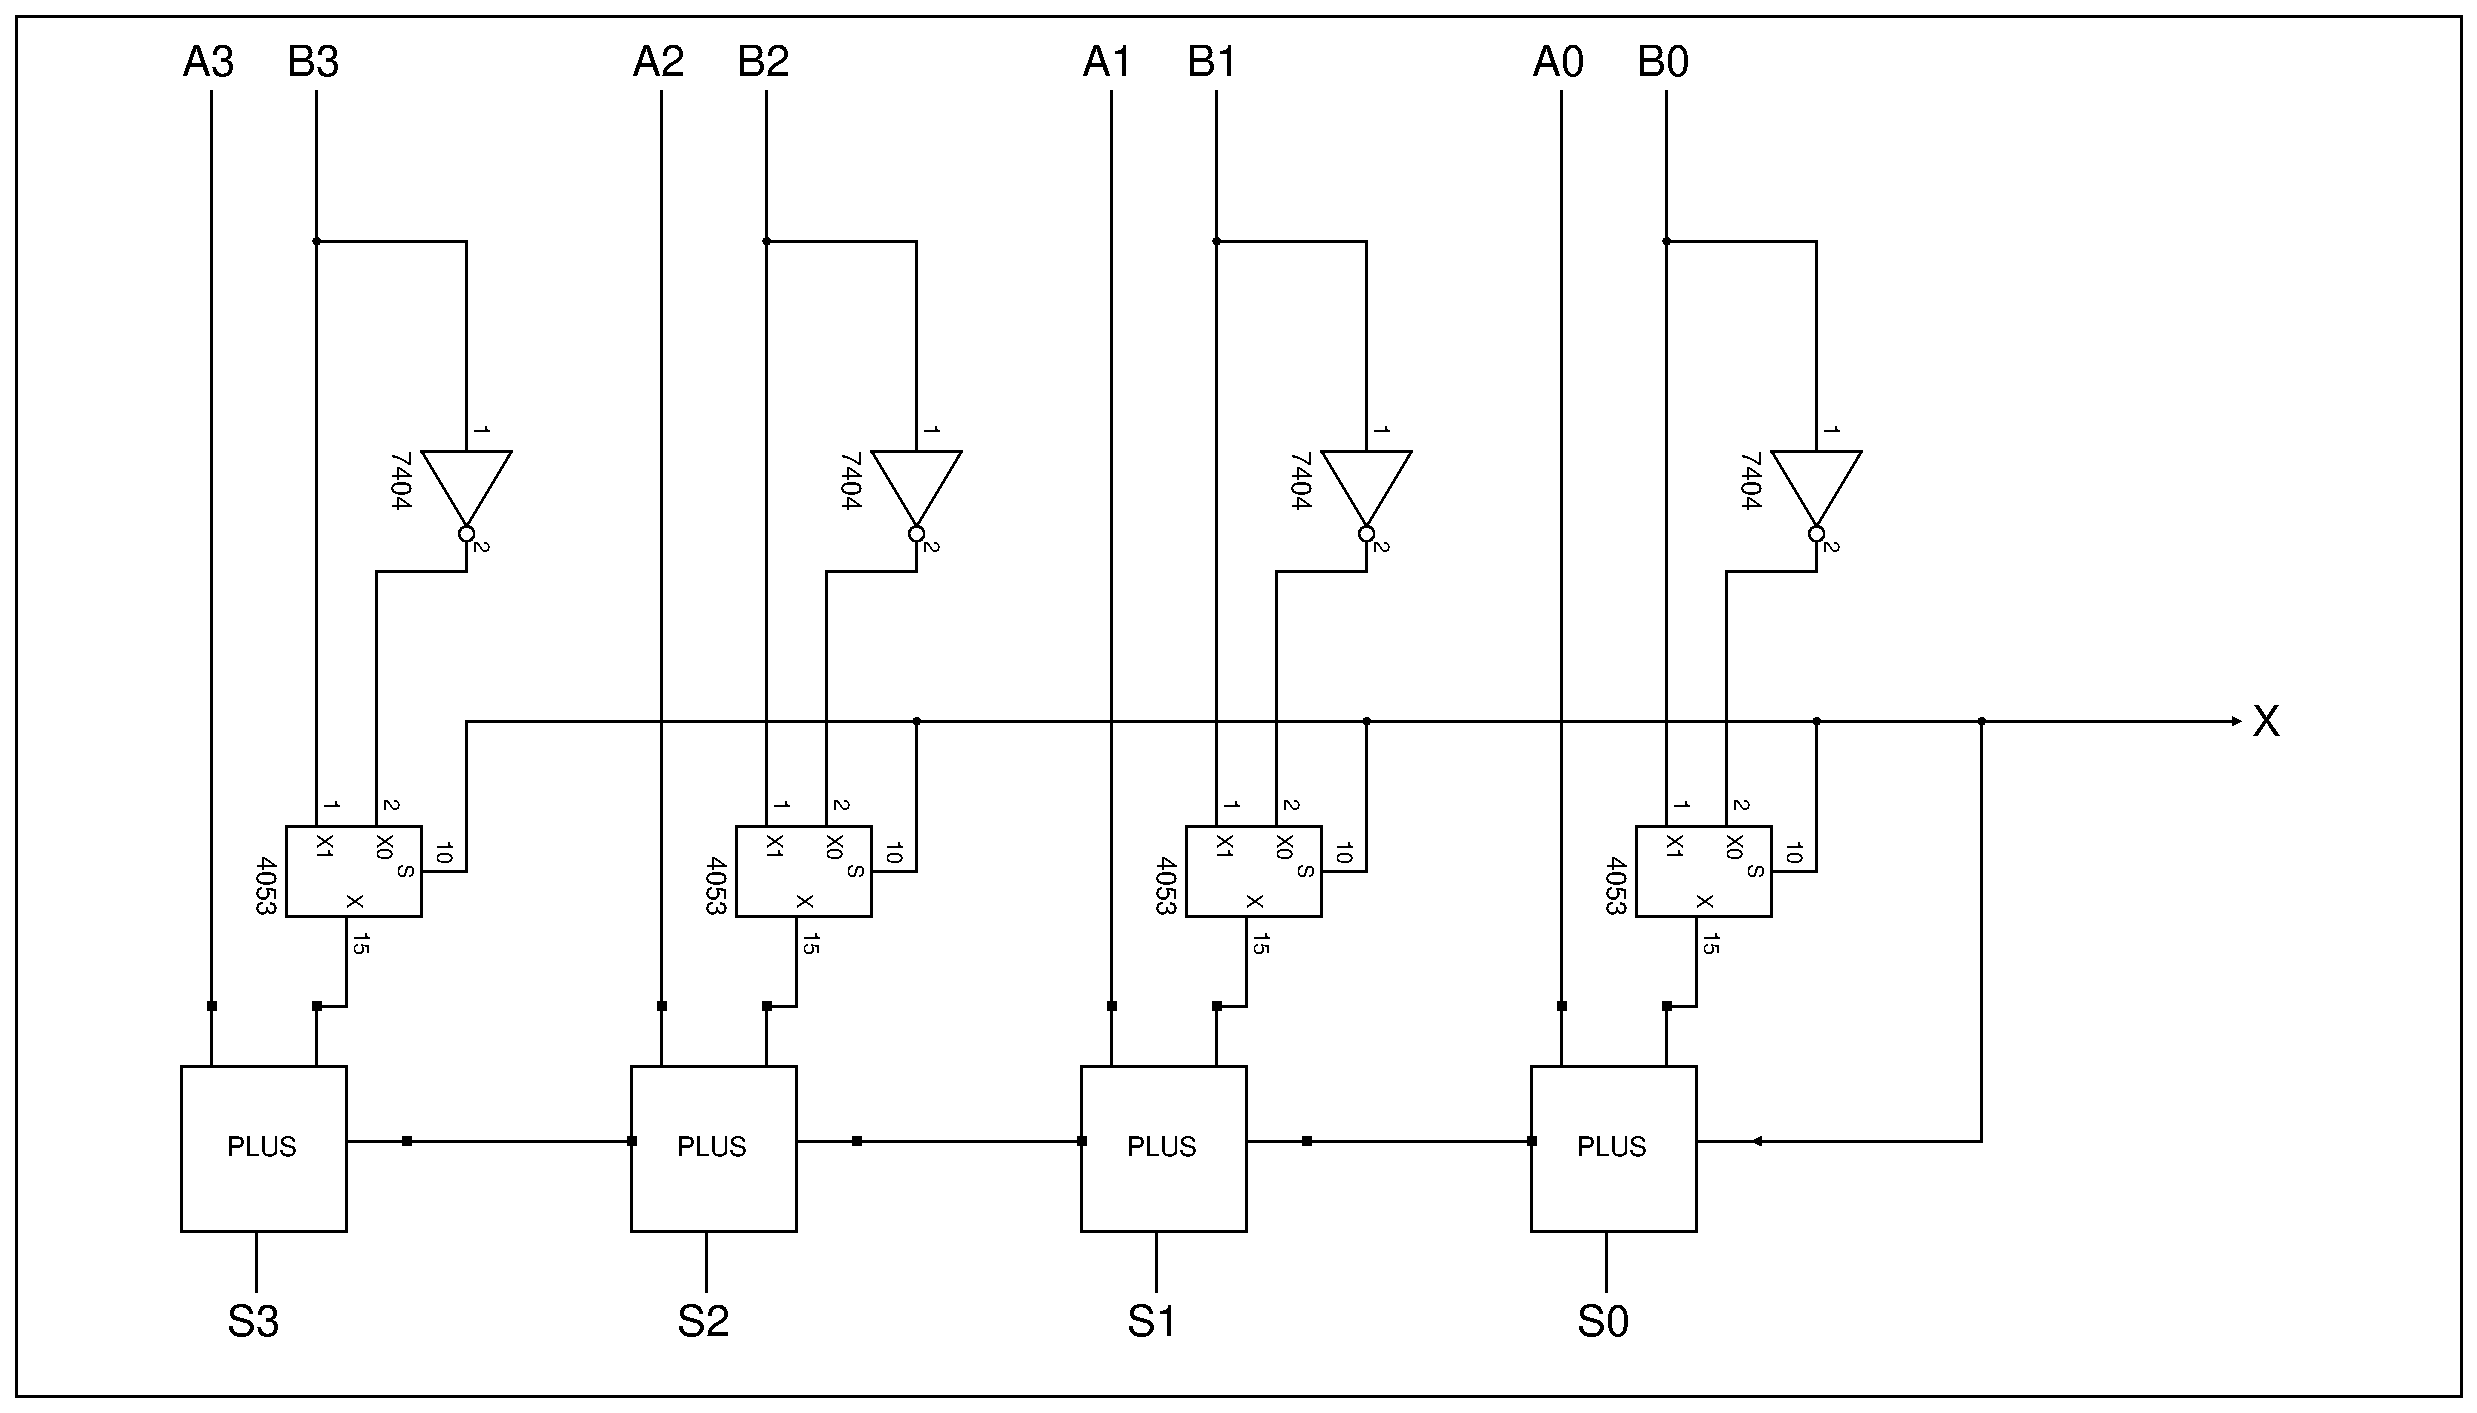
\includegraphics[width=0.5\paperwidth]{a-s.eps}
  \end{center}
\end{enumerate}

\item[3.25]
\begin{enumerate}
\item 3 gate delays
\item 3 gate delays
\item $3\times 4 = 12$ gate delays
\item $3\times 32 = 96$ gate delays
\end{enumerate}
\item[3.34]
\begin{enumerate}
\item 3
\item 4
\item 0001
\end{enumerate}
\end{enumerate}

\end{document}
